% !TeX spellcheck = en_UK

\section{Overview of Radio Interferometric Techniques}\label{section.imaging}

\pg
In this section, we will cover the difficulties introduced by the combination of sparse $uv$-coverage and weak \emph{a priori} constraints on the sky brightness distribution. While we do not need to strictly base ourselves on the RIME formalism described in \cref{section.RIME}, it remains the conceptual framework we will assume that the reader uses. For the remainder of this section, we will assume that calibration has been successfully carried out, and that we are working on the \emph{corrected visibilities}, i.e. gain-corrected visibilities. 

\pg
We will begin by linking interferometry to more concrete concepts: specifically, we will give a (very!) brief introduction to radio antennas and their characteristics. This will make the ideas and basis of radio interferometry more accessible by allowing us to explain the abstractions that interferometry relies on in terms of simpler instrumental configurations. We will then introduce the concrete problems that interferometry introduces: both a recapitulation of the venerable Zernike-van Cittert theorem \citep[cf.][]{1934Phy.....1..201V} and the problem of incomplete $uv$-coverage.


%
%\pg
%There exists a wide variety of methods used in imaging, from the venerable CLEAN algorithm\footnote{For an excellent beginner's introduction to CLEAN, the author heartily recommends \url{https://www.cv.nrao.edu/~abridle/deconvol/node7.html}} to cutting-edge compressed sensing and subspace deconvolution methods. We will begin this section by introducing a mathematical framework in which the problem of deconvolution can be understood, and proceed, from there, to discuss some of the deconvolution algorithms which can be used.
%
%\pg
%The formalism used in this section is based, in part or in whole, on that used by Cyril Tasse in [DDF paper].

\section{A Brief Introduction to Radio Astronomy}

\pg
Radio astronomy consists of observing the electromagnetic field at very long wavelengths, which means using radio dishes. These dishes measure a voltage signal, proportional to variations in the electromagnetic field in the direction of sensitivity. Achieving good sensitivity with radio dishes means having a very large collecting area - in this respect, they behave exactly the same way as optical telescopes. Similarly, when well-designed, they are diffraction-limited - this means that, once again like optical telescopes, their resolution is limited by their diameter.

\pg
However, because radio frequencies are so much lower, achieving a resolution comparable to e.g. the HST requires extremely large dishes. While there exist telescopes, both old and new, which work on this principle (from Arecibo Observatory, shown in Fig. , to the upcoming FAST telescope in China, shown in Fig. )

\begin{figure}[ht]
\centering
\begin{subfigure}{.43\textwidth}
\resizebox{\hsize}{!}{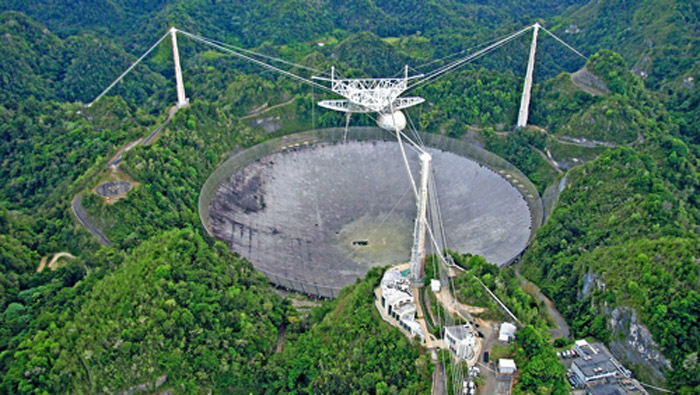
\includegraphics{images/20151101114231-0_8e7cc_c7a44aca_orig.jpg}}
\caption{\label{fig.arecibo} Arecibo telescope, in Puerto Rico.}
\end{subfigure}
\hfill
\begin{subfigure}{.43\textwidth}
\resizebox{\hsize}{!}{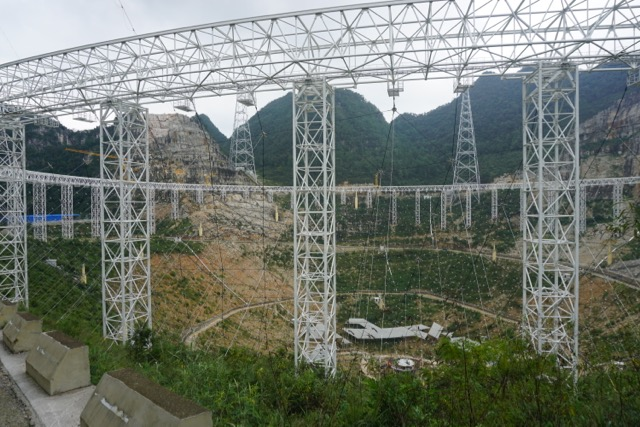
\includegraphics{images/FastTelescope_8sep2015.jpg}}
\caption{\label{fig.FAST} FAST telescope, in China}
\end{subfigure}
\caption{\label{fig.singleDishes} Examples of large single-dish radio telescopes.}
\end{figure}

\pg
Calibrating these dishes is a relatively straightforward matter - the signal loss and distortion as the dish converts the electromagnetic wave to a voltage can be described, based on the dish, either as a simple scaling factor, or a complex number (giving information on phase and amplitude errors). This loss and distortion model is referred to as the \emph{antenna gain}. Solving for these using more complex interferometric array is a problem described in Section \ref{section.calibration}.

\pg
For the remainder of this section, we will assume that calibration has been performed perfectly, and that the gain-corrections have been applied to voltage measurements. 

\section{Interferometry: Bypassing the Diffraction Limit}

\pg
There are two quantities of interest to astronomers of all stripes: sensitivity and resolution. An instrument's sensitivity is a function of its collecting area\footnote{It is also a function of technological factors, of course, but \emph{ceteris paribus}, a more sensitive telescope means a telescope with a wider collecting area}. Resolution, for well-designed instruments\footnote{By this, we mean that we assume that an instrument strives to optimise resolution.}, is limited by diffraction. This introduces issues specific to the radio domain. Radio waves, however, have very long wavelengths - often comparable to meters, rather than the 100$nm$ wavelengths of optical light. This introduces specific issues for astronomers, since achieving a resolution comparable to those of optical telescopes would require making telescopes with apertures tens of millions of times larger than those already titanic instruments!

\pg
To produce high-resolution maps of the radio sky, this technical limitation demands a technical solution. In practice, this solution consists of recourse to interferometric techniques. Indeed, interferometry can be thought of as the construction of a "sparse" dish, as illustrated in Fig.

\begin{figure}[ht]
\centering
\begin{subfigure}{.43\textwidth}
\resizebox{\hsize}{!}{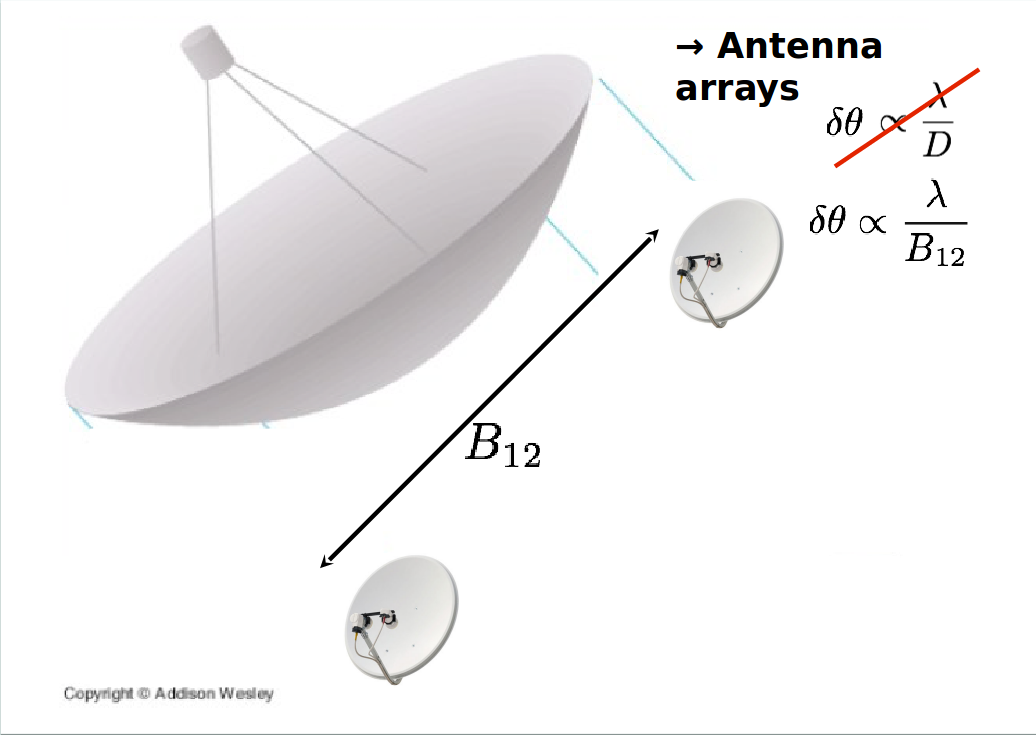
\includegraphics{images/baseline-resolution.png}}
\caption{\label{fig.baseline.image} A pair of dishes can surpass the resolution limit of its components.}
\end{subfigure}
\hfill
\begin{subfigure}{.43\textwidth}
\resizebox{\hsize}{!}{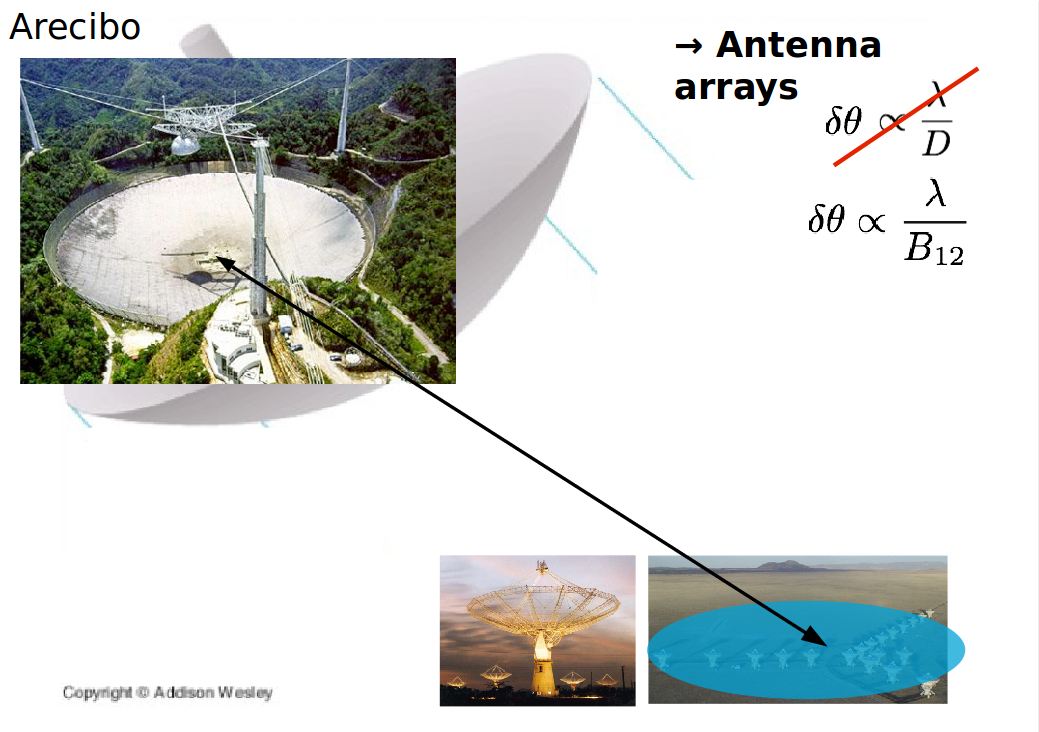
\includegraphics{images/arecibo-vla.png}}
\caption{\label{fig.arecibo.vla} With enough pairs of dishes, it is possible to synthesise a much larger dish.}
\end{subfigure}
\caption{\label{fig.aperture.synthesis} Illustration of the underlying principle of interferometry. The 27 dishes of the VLA can be thought of as "synthesising" a similar circular dish as Arecibo. This idea is the reason why radio interferometry is historically known as "aperture synthesis" in the literature of radio astronomy. Both images are copyrighted by Addison Wesley.}
\end{figure}

\pg
Of course, this improvement of resolution does not come for free. To understand the cost of interferometry, let us discuss the properties of its core component: the baseline.

\subsection{The Baseline}

\pg
To define the baseline, we must begin by considering the geometric properties of an interferometric array. For now, let us assume that we are observing the sky above the array, a practice known as drift-scanning. A baseline then consists of the vector subtraction of the positions, in 3-dimensional space, of its two constituent antennas. Note that each antenna pair therefore has 2 corresponding baselines, since for each pair of antennas A and B we have baselines AB and BA. These distance vectors are then divided by the observing wavelength to give a dimensionless set of coordinates, known as $(u,v,w)$. These coordinates define the baseline entirely. 

\subsection{The Visibility}

\pg
We have defined what a baseline corresponds to: a vector coordinate in $(u,v,w)$-space. To each baseline we associate a measurement, which we call the \emph{visibility}. 
\begin{figure}[ht]
\centering
\resizebox{\hsize}{!}{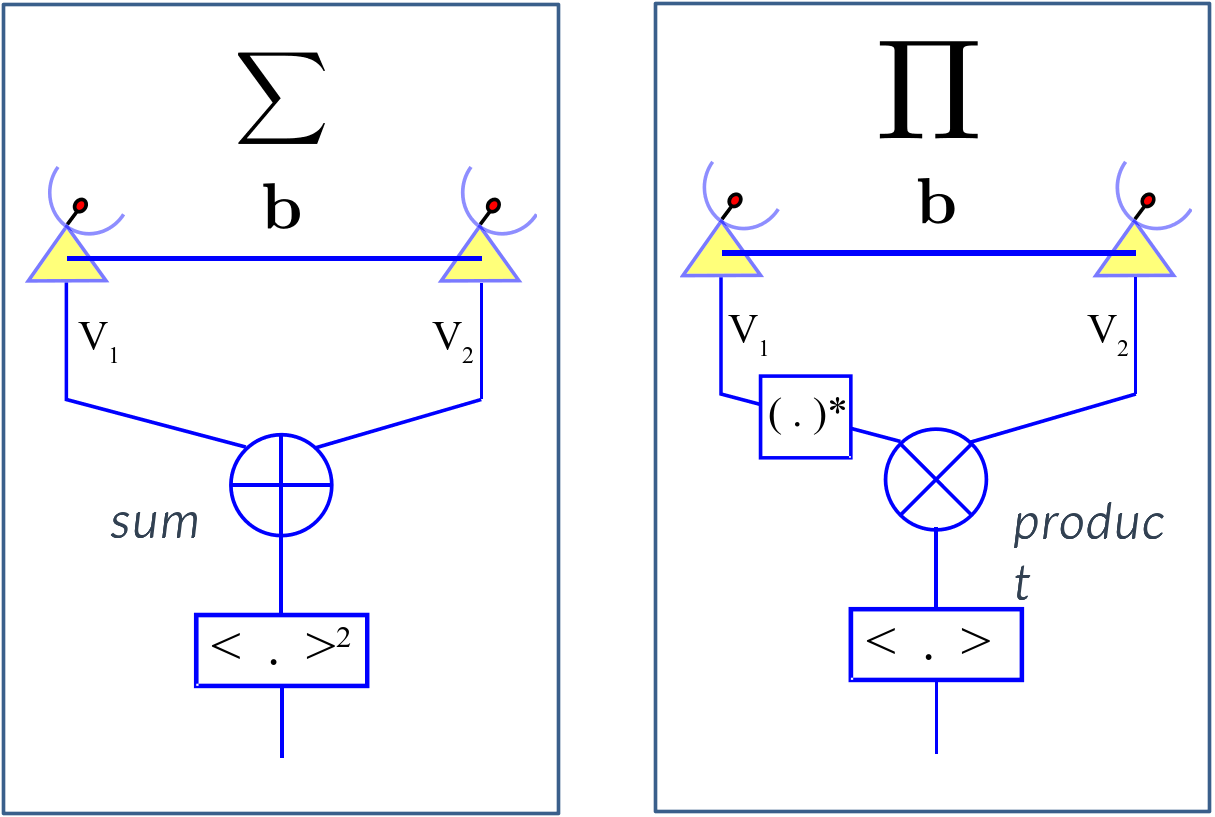
\includegraphics{images/visibility-creation.png}}
\caption{\label{fig.visibility} There are two ways to combine the voltages from two antennas into a visibility: they are sum-correlation and $\pi$-correlation. In this manuscript, we will only concern ourselves with the latter. Image credit: Julien Girard}
\end{figure}
The visibility associated with baseline $\mathbf{b}_{AB}$ is created by taking the voltage measured by antenna A, multiply it by the complex conjugate of the voltage measured by antenna B, average over the correlator dump time (i.e. the time over which the measurement is made). This scalar quantity is then multiplied by the baseline position vector. In other words:
\begin{equation}
\mathbf{b}_{AB} = V_{A} V_{B}^* \frac{\mathbf{x}_{B}-\mathbf{x}_{A}}{\nu_\mathrm{obs}}
\end{equation}

\pg
So we see that a visibility is a complex vector quantity. We also see that $\mathbf{b}_{AB} = \mathbf{b}_{BA}^*$: the information of the visibility associated with baseline BA is contained in the visibility associated with baseline AB. This means that in practice, only half of the visibilities ever need be stored. What does the visibility measurement correspond to?
\begin{figure}[ht]
\centering
\resizebox{\hsize}{!}{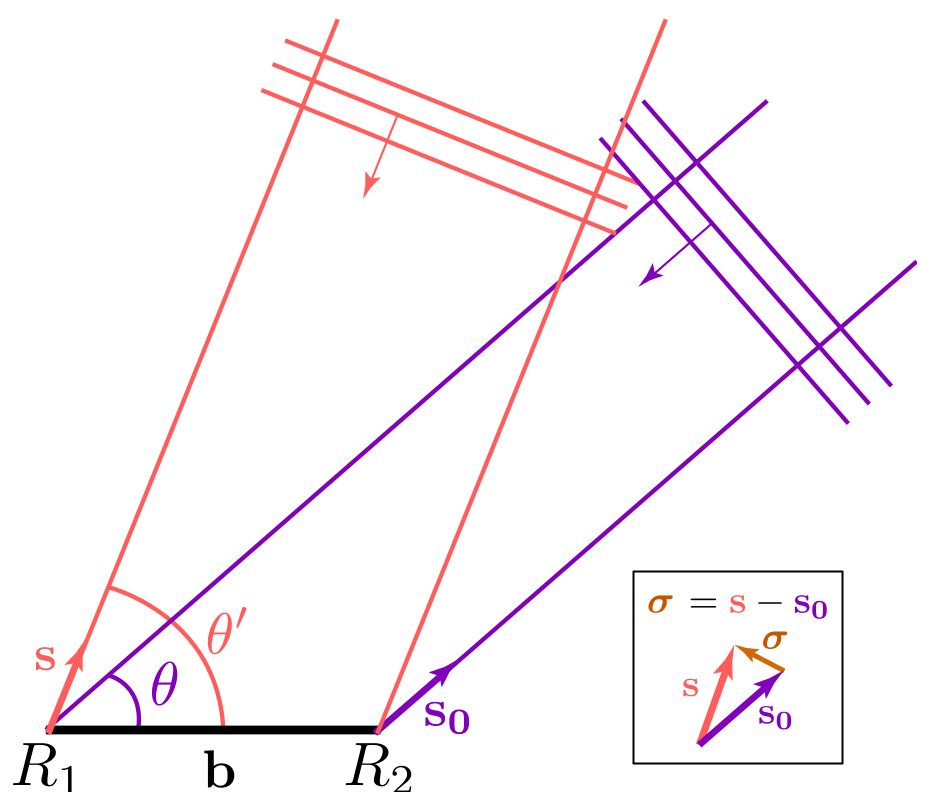
\includegraphics{images/visibility-measure.png}}
\caption{\label{fig.visibility.measure} Here, we assume that there are only two sources in the sky whose signal can be measured by our antennas. The final visibility is the sum of the visibilities associated with each individual source. Image credit: Julien Girard}
\end{figure}

\pg
The signals from various sources are additive in both antennas. Provided that the signal from both sources is coherent when observed by the dishes, the correlation between the total voltages will simply be the sum of the voltage correlations associated with individual sources - i.e. the interferometric signal from different sources are additive.

\pg
Note that in Fig. \ref{fig.visibility.measure}, neither source is at the zenith. We thus see that the \emph{effective baseline} which sees each source is in fact shorter than the \emph{physical baseline}. This can be corrected by digitally adding a phase delay in each antenna (or, in older interferometers, by playing with the cable length between each dish and the correlator) - this is in fact how interferometric arrays are pointed.

\subsection{The $uv$-plane}

\pg
In general, interferometric design is such that the $w$ component of visibilities' $(u,v,w)$ coordinates is negligible (or can be put in a frame of reference where it can usually be approximated as such). Radio astronomers tend to thus talk of a $uv$-plane rather than $uvw$-space to describe the space where visibilities live. The set of $uv$-values for all the baselines of an interferometric array is known as its $uv$-coverage, and defines the array's properties entirely.

\pg
For the VLA, for example, the $uv$-coverage when observing the zenith will be as shown in Fig. \ref{fig.vla.uvcoverage}.

\begin{figure}[ht]
\centering
\resizebox{\hsize}{!}{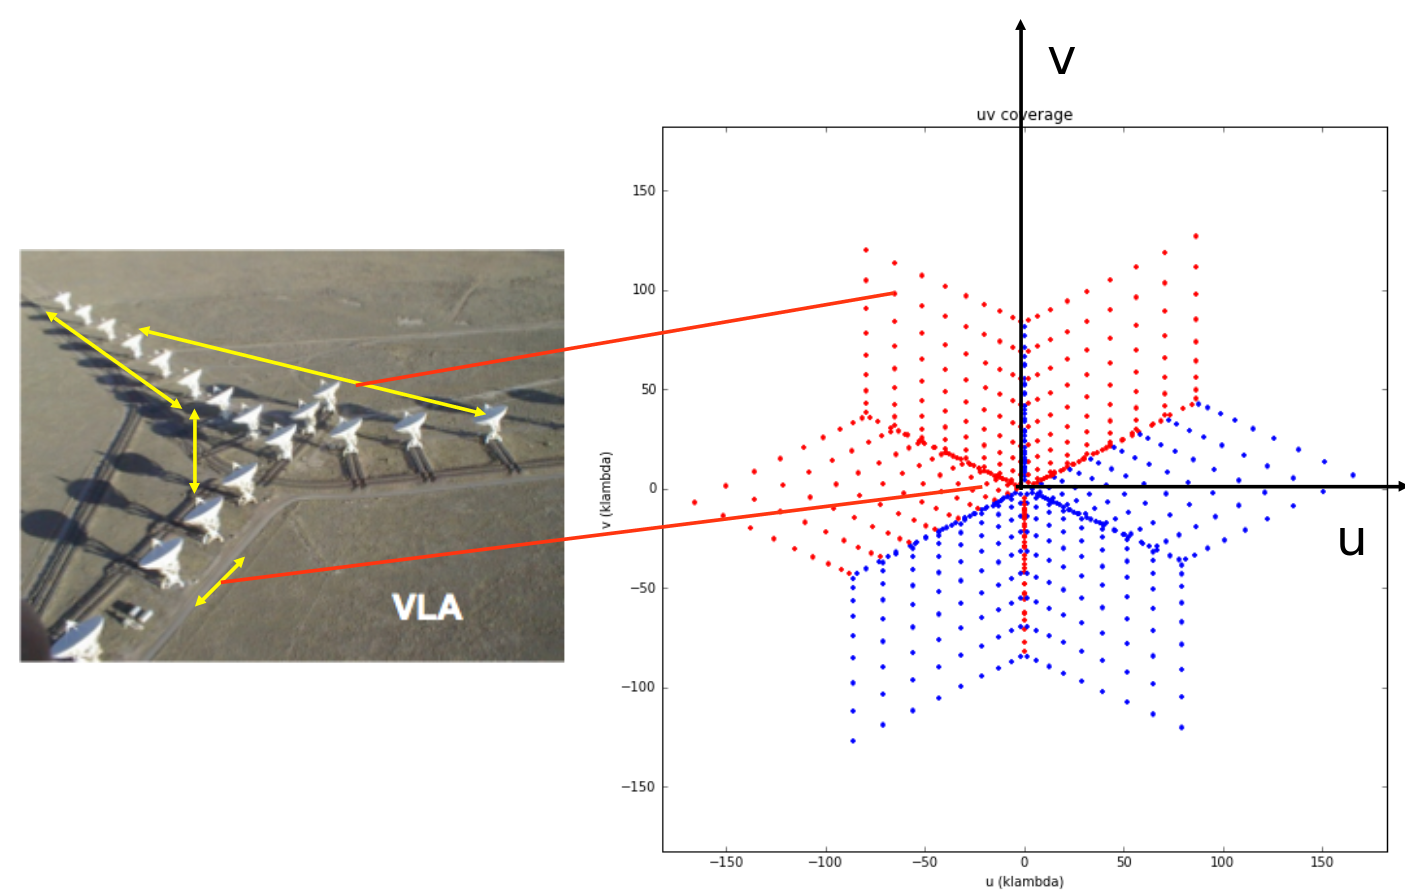
\includegraphics{images/vla-uvcoverage.png}}
\caption{\label{fig.vla.uvcoverage} The VLA contains 27 radio dishes placed as shown above. Each antenna pair between those 27 gives two single baselines, here, one red and one blue. Image credit: Julien Girard}
\end{figure}

%\pg
%The more points an array has in $uv$-space, the greater its $uv$-coverage and the better it will observe. This coverage can be improved for free in two main ways: firstly, the use of a technique known as supersynthesis (since the interferometer "synthesises" a dish at any given time, by assuming that the sky does not evolve over a certain time frame, we can treat different times as measurements of the same sky) and taking advantage of the frequency-dependence of $uv$-coordinates.The impact of both practices will be described in greater detail in \ref{sec.imag.psf}, but know that "$uv$-tracks" simply correspond to the $uv$-coverage of an interferometer observing over some period of time.

\pg
Individual antennas of an array can be pointed mechanically, and so the impact of pointing the interferometric array in a given direction can be minimised. But what happens to the array itself? It is useful here to go back to the illustration of Fig. \ref{fig.arecibo.vla}. Think of each dish in the array representing a "filled" segment of a massive but empty dish. By projecting our observation in a given direction, this dish goes from circular to elliptical.
\begin{figure}[ht]
\centering
\begin{subfigure}{.40\textwidth}
\resizebox{\hsize}{!}{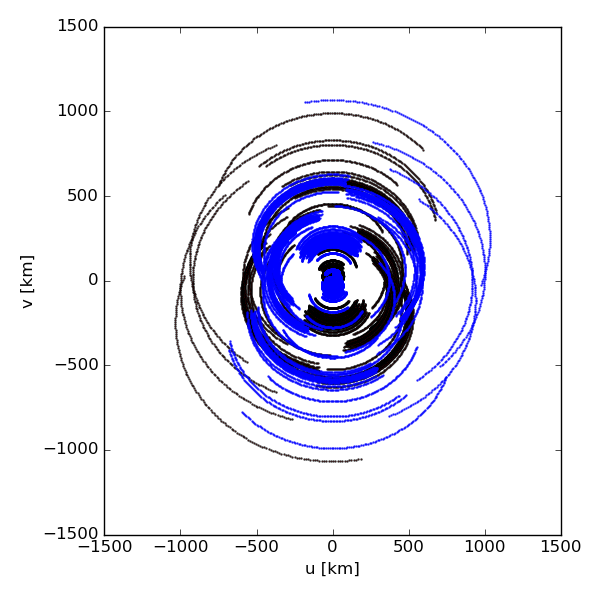
\includegraphics{images/lofar-uvcoverage-zenith.png}}
\caption{\label{fig.lofar.uvcoverage.zenith} $uv$-coverage of an 8-hour LOFAR observation when pointing at zenith..}
\end{subfigure}
\hfill
\begin{subfigure}{.40\textwidth}
\resizebox{\hsize}{!}{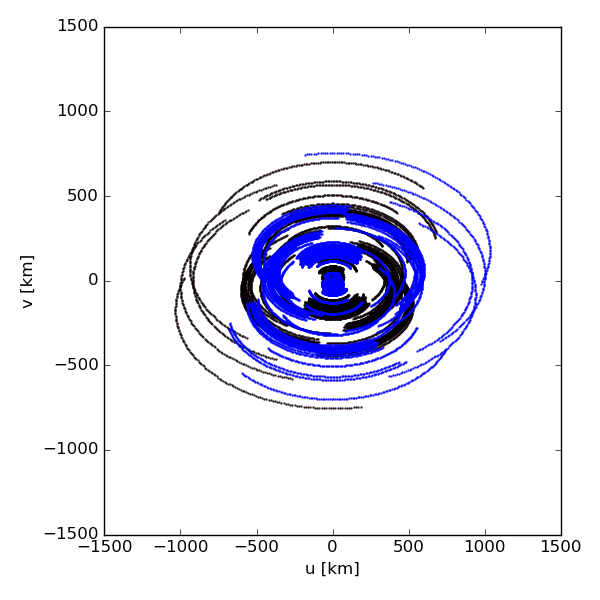
\includegraphics{images/lofar-uvcoverage-elsewhere.png}}
\caption{\label{fig.lofar.uvcoverage.elsewhere} $uv$-coverage of an 8-hour LOFAR observation when pointing 45 degrees away from zenith.}
\end{subfigure}
\caption{\label{fig.uvcoverage.lofar} Effect of array pointing on $uv$-coverage. By pointing the array 45 degrees in the $v$-axis, the array's $uv$-coverage (and thus maximum resolution) is decreased along the $v$-axis.}
\end{figure}


\subsection{The Point-Spread Function}\label{sec.imag.psf}

\pg
So far, we have seen that the purpose an interferometric array is to overcome the diffraction limit of single-dish antennas. We have described visibilities, which are the quantities measured by an interferometric array. What remains is to describe how these measurements are used to go make images of the sky.

\pg
Assuming that all the antennas in an array are equivalent and perfectly calibrated, the van Cittert-Zernike theorem (\citepads{1934Phy.....1..201V}, covered in \citepads{2001isra.book.....T}) allows us to equate a visibility with a single Fourier mode of the plane tangent to the sky where the instrument is pointed. This direction is called the \emph{phase centre}, because digital phase shifts are introduced between antenna voltages before averaging so as to point each visibility in this direction. 

\subsection{From Dirty to Clean: Mitigating the PSF}
